\documentclass[a4paper,twoside,7pt]{book}

\usepackage{latexsym}%symbole
\usepackage[empty]{fullpage}
\usepackage{titlesec}%alternatywne sekcje tytułowe
\usepackage{marvosym}%wiecej symboli
\usepackage[usenames,dvipsnames]{color}
\usepackage{verbatim}%wyświetlanie kodu
\usepackage{enumitem}%zmienianie layoutu
\usepackage[hidelinks]{hyperref}%?!?!?!
\usepackage{fancyhdr}%heders and footers
\usepackage[english]{babel}%znaki lokalne?
\usepackage{tabularx}% tabeli 
\usepackage{multicol}% wiele column
\usepackage{minted}% syntax hilighting
\input{glyphtounicode}

\usepackage{baskervillef}
\usepackage[T1]{fontenc}
%flow chatry
\usepackage{tikz}
\usetikzlibrary{shapes.geometric, arrows}
\usepackage{amssymb}
\usepackage{float}
\usepackage{pgf}

\pagestyle{fancy}
\fancyhf{} 
\fancyfoot[OR]{\thepage}
\fancyfoot[EL]{\thepage}
\setlength{\footskip}{5pt}
\renewcommand{\headrulewidth}{0pt}
\renewcommand{\footrulewidth}{0pt}

\usepackage[left=0.5in,right=0.5in,top=0.5in,bottom=0.5in,inner=2.6cm]{geometry}

\urlstyle{same}

%\raggedbottom
\raggedright
\setlength{\tabcolsep}{0in}

\titleformat{\section}{
  \it\vspace{3pt}
}{}{0em}{}[\color{black}\titlerule\vspace{-5pt}]

\pdfgentounicode=1
%flowchatrts shapes

\definecolor{1}{RGB}{128, 147, 241}
\definecolor{2}{RGB}{114, 221, 247}
\definecolor{3}{RGB}{179, 136, 235}
\definecolor{4}{RGB}{247, 174, 248}

\tikzstyle{startstop} = [ellipse, rounded corners, minimum width=2cm, minimum height=1cm,text centered, draw=black,thick,fill=4]
\tikzstyle{io} = [trapezium,trapezium stretches=true,trapezium left angle=70,trapezium right angle=110,thick,minimum width=1cm,minimum height=0.85cm, text centered, draw=black,fill=1]
\tikzstyle{process} = [rectangle,minimum width=1cm,minimum height=0.85cm,text centered,draw=black,thick,fill=2]
\tikzstyle{decision} = [diamond,minimum width=1cm, minimum height=1cm, text centered, draw=black, fill=3,thick]
\tikzstyle{arrow} = [thick,->,>=stealth]
\tikzstyle{none} = [coordinate]
\tikzstyle{con} = [thick]

\begin{document}
\raggedcolumns
\begin{center}
    \begin{multicols}{2}
    \begin{flushleft}
    \large{Tymon Łazowy 3D nr.09} \\
    \end{flushleft}
    
    \begin{flushright}
    \large{29.09.2023}\\
    \end{flushright}
    \end{multicols}
    {\LARGE Sprawozdanie z informatyki nr 2} \\ \vspace{0pt}
\end{center}

\section{Treść zadanie}
\begin{center}
\large{Programownie część Druga}\\

\begin{itemize}[ label={}]
    \normalsize{\item{
    {2.1 - Program przeliczający waluty}{} \\
    {2.2 - Program obliczający pola i obwody 4 figur geometrycznych foremnych}{} \\
    {2.3 - Program sprawdzający ile jest cyfr w liczbie całkowitej z przedziału <0,miliard> \\
    {2.4 - Liczby podzielne z przedziału}{} \\
    {2.5 - Średnia arytmetyczna z n liczb podanych przez użytkownika}{} \\
    {2.6 - Wyświetlenie i zliczenie wszystkich naturalnych liczb trzycyfrowych w których suma
cyfr wynosi n}{} \\
    {2.7 - Przerób program 2.6 tak, aby działał w pętli}{} \\
    {2.8 - Średnia arytmetyczna z n liczb dwucyfrowych, dodatnich podanych przez użytkownika}{} \\
    {2.9 - Program obliczający NWD i NWW 2 liczb a i b}{} \\
    {2.10 - Tabliczka mnożenia od-do}{} \\
    {2.11 - Szukanie minimalnej liczby z ciągu liczb dwucyfrowych podawanych przez użytkownika}{}\\
    {2.12 - Program obliczający NWD z 2 liczb(odejmowanie)}{}\\
    {2.13 - Obliczanie n! dla liczby naturalnej n>=0 – algorytm iteracyjny}{}\\
    {2.14 - Obliczanie wartości n-tego wyrazu ciągu Fibonacciego (n>=1) – algorytm iteracyjny}{}\\
    {2.15 - Sprawdzanie czy liczba n (n>0) jest liczbą pierwszą}{}\\
    {2.16 -  Suma cyfr liczby całkowitej n (n>0)}{}\\
}}}
\end{itemize}

\end{center}
%---------------------PROPONOWANE ROZWIĄZANIA-------------

\section{Proponowane rozwiązania}
\subsection*{2.1}
%----------------2.1------------------
\subsection*{dis()}
\begin{multicols}{2}
  \begin{flushleft}
\begin{minted}[framesep=1mm, baselinestretch=1.,linenos]{cpp}
dis(char a)
{switch (a)
{case 'E':
	cout<<"EUR:"<<saldo/e<<endl;	
    break;
case 'U':
	cout<<"USD:"<<saldo/u<<endl;	
	break;
case 'F':
	cout<<"CHF:"<<saldo/f<<endl;	
	break;
case 'P':
	cout<<"PLN:"<<saldo/p<<endl;	
    break;
}}

\end{minted}
    \end{flushleft}
D: \\
Saldo, kwota pieniedzy $\in$ $\mathbb{R}$\\
c, waluta $\in$ \{u,f,p,e\}\\
W: strumień, saldo w innych walutach $\in$ $\mathbb{R}$
    \begin{flushright}
    \begin{minted}[framesep=1mm, baselinestretch=1.,linenos]{cpp}
dis(char a)
{switch (a)
{case 'E':
	cout<<"EUR:"<<saldo/e<<endl;	
    break;
case 'U':
	cout<<"USD:"<<saldo/u<<endl;	
	break;
case 'F':
	cout<<"CHF:"<<saldo/f<<endl;	
	break;
case 'P':
	cout<<"PLN:"<<saldo/p<<endl;	
    break;
}}

\end{minted}
    \end{flushright}
\end{multicols}
\newpage
\subsection*{Main}
\begin{multicols}{2}
  \begin{flushleft}
\begin{minted}[framesep=1mm, baselinestretch=1.,linenos]{python}
import msvcrt
def dis(argument):
    switcher = {
        'E': print("EUR:",saldo/e,'\n'),
        'U': print("USD:",saldo/u,'\n'),
        'F': print("CHF:",saldo/f,'\n'),
        'P': print("PLN:",saldo/p,'\n'),
    }
e=4;u=3;f=5;p=1
saldo=int(input('Ile masz pieniedzy:'))
print('w jakiej walucie')
c=msvcrt.getche().upper()
print(c)
match c:
    case b'E': 
        saldo=saldo*e; dis('E'),
    case b'U':
        saldo=saldo*u; dis('U'),
    case b'F':
        saldo=saldo*f; dis('F'),
    case b'P':
        saldo=saldo*p; dis('p'),
\end{minted}
    \end{flushleft}
D: \\
Saldo, kwota pieniedzy $\in$ $\mathbb{R}$\\
c, waluta $\in$ \{u,f,p,e\}\\
W: strumień, saldo w innych walutach $\in$ $\mathbb{R}$
    \begin{flushright}
    \begin{minted}[framesep=1mm, baselinestretch=1.,linenos]{python}
import msvcrt
def dis(argument):
    switcher = {
        'E': print("EUR:",saldo/e,'\n'),
        'U': print("USD:",saldo/u,'\n'),
        'F': print("CHF:",saldo/f,'\n'),
        'P': print("PLN:",saldo/p,'\n'),
    }
e=4;u=3;f=5;p=1
saldo=int(input('Ile masz pieniedzy:'))
print('w jakiej walucie')
c=msvcrt.getche().upper()
print(c)
match c:
    case b'E': 
        saldo=saldo*e; dis('E'),
    case b'U':
        saldo=saldo*u; dis('U'),
    case b'F':
        saldo=saldo*f; dis('F'),
    case b'P':
        saldo=saldo*p; dis('p'),
\end{minted}
    \end{flushright}
\end{multicols}

\subsection*{2.2}
%----------------2.2------------------
\begin{multicols}{2}
  \begin{flushleft}
\begin{minted}[framesep=1mm, baselinestretch=1.,linenos]{cpp}
int a;char fig; 
cout<<"podaj długość boku:"<<endl;
cin>>a;cout<<"dostępne figury:\n1.kwadrat\
\n2.trójkąt\n3.pięcokąt\n4.sześciokąt";
fig=getch();
switch (fig)
{case '1':
cout<<"\nobwód jest równy "<<a*4<<"\
a pole "<<a*a;break;
case '2':
cout<<"\nobwód jest równy "<<a*3<<"\
a pole "<<a*a*sqrt(3)/4;break;
case '3':
cout<<"\nobwód jest równy "<<a*5<<"\
a pole "<<(sqrt(25+10*sqrt(5))/4)*a*a;break;
case '4':
cout<<"\nobwód jest równy "<<a*6<<"\
a pole "<<(a*a*sqrt(3)/4)*6;break;        
default:
cout<<"podana opcja jest zła";break;}
\end{minted}
    \end{flushleft}
D: a, długość boku >= 0 $\in$ $\mathbb{R}$\\
fig, typ figury $\in$ \{1;2;3;4\}\\
W: p, pole >= 0 $\in$ $\mathbb{R}$\\
obw, obwód >=0 $\in$ $\mathbb{R}$
    \begin{flushright}
    \begin{minted}[framesep=1mm, baselinestretch=1.,linenos]{cpp}
int a;char fig; 
cout<<"podaj długość boku:"<<endl;
cin>>a;cout<<"dostępne figury:\n1.kwadrat\
\n2.trójkąt\n3.pięcokąt\n4.sześciokąt";
fig=getch();
switch (fig)
{case '1':
cout<<"\nobwód jest równy "<<a*4<<"\
a pole "<<a*a;break;
case '2':
cout<<"\nobwód jest równy "<<a*3<<"\
a pole "<<a*a*sqrt(3)/4;break;
case '3':
cout<<"\nobwód jest równy "<<a*5<<"\
a pole "<<(sqrt(25+10*sqrt(5))/4)*a*a;break;
case '4':
cout<<"\nobwód jest równy "<<a*6<<"\
a pole "<<(a*a*sqrt(3)/4)*6;break;        
default:
cout<<"podana opcja jest zła";break;}
\end{minted}
    \end{flushright}    
\end{multicols}
\newpage

\subsection*{2.3}
%----------------2.3------------------
\begin{multicols}{2}
  \begin{flushleft}
\renewcommand{\thefigure}{3}
\begin{figure}[H]
    \centering 
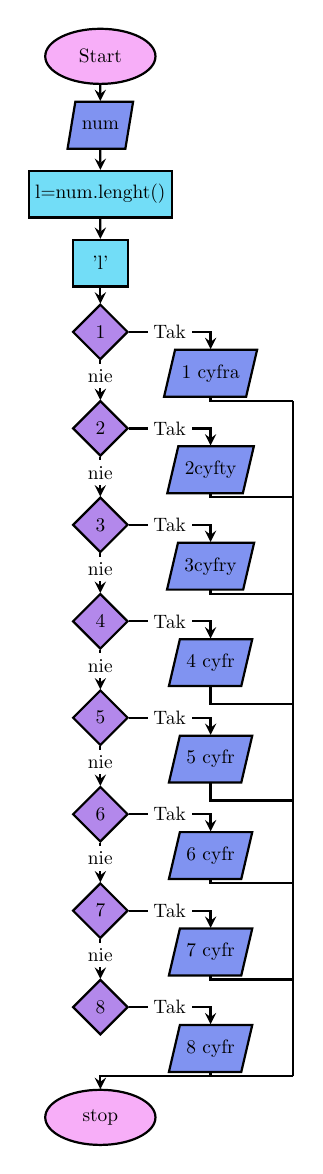
\begin{tikzpicture}[scale=0.7,transform shape]
		\node [style=startstop] (0) at (0, 0) {Start};
		\node [style=io] (1) at (0, -1.25) {num};
		\node [style=process] (3) at (0, -3.75) {'l'};
		\node [style=decision] (4) at (0, -5) {1};
		\node [style=decision] (5) at (0, -6.75) {2};
		\node [style=decision] (6) at (0, -8.5) {3};
		\node [style=decision] (7) at (0, -10.25) {4};
		\node [style=process] (8) at (0, -2.5) {l=num.lenght()};
		\node [style=decision] (9) at (0, -12) {5};
		\node [style=decision] (10) at (0, -13.75) {6};
		\node [style=decision] (11) at (0, -15.5) {7};
		\node [style=decision] (12) at (0, -17.25) {8};
		\node [style=io] (14) at (2, -5.75) {1 cyfra};
		\node [style=io] (15) at (2, -7.5) {2cyfty};
		\node [style=io] (16) at (2, -9.25) {3cyfry};
		\node [style=io] (17) at (2, -11) {4 cyfr};
		\node [style=io] (18) at (2, -12.75) {5 cyfr};
		\node [style=io] (19) at (2, -14.5) {6 cyfr};
		\node [style=io] (20) at (2, -16.25) {7 cyfr};
		\node [style=io] (21) at (2, -18) {8 cyfr};
		\node [style=startstop] (22) at (0, -19.25) {stop};
		\node [style=none] (23) at (3.5, -6.25) {};
		\node [style=none] (24) at (3.5, -8) {};
		\node [style=none] (25) at (3.5, -9.75) {};
		\node [style=none] (26) at (3.5, -11.75) {};
		\node [style=none] (27) at (3.5, -13.5) {};
		\node [style=none] (28) at (3.5, -15) {};
		\node [style=none] (29) at (3.5, -16.75) {};
		\node [style=none] (30) at (3.5, -18.5) {};

%\draw [arrow] (c3) -- (c4)node[pos=0.4,fill=white,inner sep=3]{nie};
%\draw [arrow] (c1) -| (p1)node[pos=0.25,fill=white,inner sep=3]{Tak};

		\draw [style=arrow] (0) to (1);
		\draw [style=arrow] (1) to (8);
		\draw [style=arrow] (8) to (3);
		\draw [style=arrow] (3) to (4);
		\draw [style=arrow] (4) -- (5)node[pos=0.4,fill=white,inner sep=3]{nie};
		\draw [style=arrow] (5) -- (6)node[pos=0.4,fill=white,inner sep=3]{nie};
		\draw [style=arrow] (6) -- (7)node[pos=0.4,fill=white,inner sep=3]{nie};
		\draw [style=arrow] (7) -- (9)node[pos=0.4,fill=white,inner sep=3]{nie};
		\draw [style=arrow] (9) -- (10)node[pos=0.4,fill=white,inner sep=3]{nie};
		\draw [style=arrow] (10) -- (11)node[pos=0.4,fill=white,inner sep=3]{nie};
		\draw [style=arrow] (11) -- (12)node[pos=0.4,fill=white,inner sep=3]{nie};
		\draw [style=arrow] (4) -| (14)node[pos=0.25,fill=white,inner sep=3]{Tak};
		\draw [style=arrow] (5) -| (15)node[pos=0.25,fill=white,inner sep=3]{Tak};
		\draw [style=arrow] (6) -| (16)node[pos=0.25,fill=white,inner sep=3]{Tak};
		\draw [style=arrow] (7) -| (17)node[pos=0.25,fill=white,inner sep=3]{Tak};
		\draw [style=arrow] (9) -| (18)node[pos=0.25,fill=white,inner sep=3]{Tak};
		\draw [style=arrow] (10) -| (19)node[pos=0.25,fill=white,inner sep=3]{Tak};
		\draw [style=arrow] (11) -| (20)node[pos=0.25,fill=white,inner sep=3]{Tak};
		\draw [style=arrow] (12) -| (21)node[pos=0.25,fill=white,inner sep=3]{Tak};
		\draw [style=con] (14) |- (23.center);
		\draw [style=con] (15) |- (24.center);
		\draw [style=con] (16) |- (25.center);
		\draw [style=con] (17) |- (26.center);
		\draw [style=con] (18) |- (27.center);
		\draw [style=con] (19) |- (28.center);
		\draw [style=con] (20) |- (29.center);
		\draw [style=con] (21) |- (30.center);
		\draw [style=con] (23.center) to (30.center);
		\draw [style=arrow] (30.center) -| (22);
\end{tikzpicture}
\caption{2.3 flowchart}
    \label{flow3}
\end{figure}
    \end{flushleft}
D: num, ciąg cyfra $\in$ $\mathbb{N}_0$\\
W: l, liczba cyfr $\in$ $\mathbb{N}_0$
    \begin{flushright}
    \renewcommand{\thefigure}{3}
\begin{figure}[H]
    \centering 
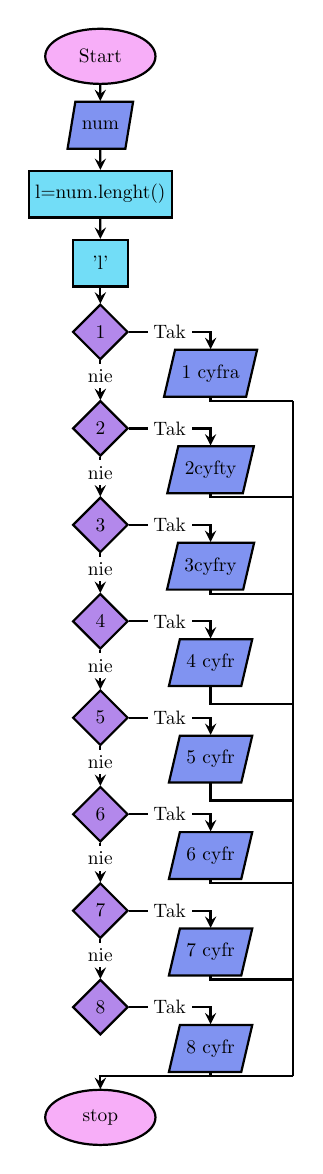
\begin{tikzpicture}[scale=0.7,transform shape]
		\node [style=startstop] (0) at (0, 0) {Start};
		\node [style=io] (1) at (0, -1.25) {num};
		\node [style=process] (3) at (0, -3.75) {'l'};
		\node [style=decision] (4) at (0, -5) {1};
		\node [style=decision] (5) at (0, -6.75) {2};
		\node [style=decision] (6) at (0, -8.5) {3};
		\node [style=decision] (7) at (0, -10.25) {4};
		\node [style=process] (8) at (0, -2.5) {l=num.lenght()};
		\node [style=decision] (9) at (0, -12) {5};
		\node [style=decision] (10) at (0, -13.75) {6};
		\node [style=decision] (11) at (0, -15.5) {7};
		\node [style=decision] (12) at (0, -17.25) {8};
		\node [style=io] (14) at (2, -5.75) {1 cyfra};
		\node [style=io] (15) at (2, -7.5) {2cyfty};
		\node [style=io] (16) at (2, -9.25) {3cyfry};
		\node [style=io] (17) at (2, -11) {4 cyfr};
		\node [style=io] (18) at (2, -12.75) {5 cyfr};
		\node [style=io] (19) at (2, -14.5) {6 cyfr};
		\node [style=io] (20) at (2, -16.25) {7 cyfr};
		\node [style=io] (21) at (2, -18) {8 cyfr};
		\node [style=startstop] (22) at (0, -19.25) {stop};
		\node [style=none] (23) at (3.5, -6.25) {};
		\node [style=none] (24) at (3.5, -8) {};
		\node [style=none] (25) at (3.5, -9.75) {};
		\node [style=none] (26) at (3.5, -11.75) {};
		\node [style=none] (27) at (3.5, -13.5) {};
		\node [style=none] (28) at (3.5, -15) {};
		\node [style=none] (29) at (3.5, -16.75) {};
		\node [style=none] (30) at (3.5, -18.5) {};

%\draw [arrow] (c3) -- (c4)node[pos=0.4,fill=white,inner sep=3]{nie};
%\draw [arrow] (c1) -| (p1)node[pos=0.25,fill=white,inner sep=3]{Tak};

		\draw [style=arrow] (0) to (1);
		\draw [style=arrow] (1) to (8);
		\draw [style=arrow] (8) to (3);
		\draw [style=arrow] (3) to (4);
		\draw [style=arrow] (4) -- (5)node[pos=0.4,fill=white,inner sep=3]{nie};
		\draw [style=arrow] (5) -- (6)node[pos=0.4,fill=white,inner sep=3]{nie};
		\draw [style=arrow] (6) -- (7)node[pos=0.4,fill=white,inner sep=3]{nie};
		\draw [style=arrow] (7) -- (9)node[pos=0.4,fill=white,inner sep=3]{nie};
		\draw [style=arrow] (9) -- (10)node[pos=0.4,fill=white,inner sep=3]{nie};
		\draw [style=arrow] (10) -- (11)node[pos=0.4,fill=white,inner sep=3]{nie};
		\draw [style=arrow] (11) -- (12)node[pos=0.4,fill=white,inner sep=3]{nie};
		\draw [style=arrow] (4) -| (14)node[pos=0.25,fill=white,inner sep=3]{Tak};
		\draw [style=arrow] (5) -| (15)node[pos=0.25,fill=white,inner sep=3]{Tak};
		\draw [style=arrow] (6) -| (16)node[pos=0.25,fill=white,inner sep=3]{Tak};
		\draw [style=arrow] (7) -| (17)node[pos=0.25,fill=white,inner sep=3]{Tak};
		\draw [style=arrow] (9) -| (18)node[pos=0.25,fill=white,inner sep=3]{Tak};
		\draw [style=arrow] (10) -| (19)node[pos=0.25,fill=white,inner sep=3]{Tak};
		\draw [style=arrow] (11) -| (20)node[pos=0.25,fill=white,inner sep=3]{Tak};
		\draw [style=arrow] (12) -| (21)node[pos=0.25,fill=white,inner sep=3]{Tak};
		\draw [style=con] (14) |- (23.center);
		\draw [style=con] (15) |- (24.center);
		\draw [style=con] (16) |- (25.center);
		\draw [style=con] (17) |- (26.center);
		\draw [style=con] (18) |- (27.center);
		\draw [style=con] (19) |- (28.center);
		\draw [style=con] (20) |- (29.center);
		\draw [style=con] (21) |- (30.center);
		\draw [style=con] (23.center) to (30.center);
		\draw [style=arrow] (30.center) -| (22);
\end{tikzpicture}
\caption{2.3 flowchart}
    \label{flow3}
\end{figure}
    \end{flushright}    
\end{multicols}
\subsection*{2.4}
%----------------2.4------------------
\begin{multicols}{2}
  \begin{flushleft}
\begin{minted}[framesep=1mm, baselinestretch=1.,linenos]{cpp}
cout<<"ile jest liczb podzielnych\
przez c w przdziale a-b"<<endl;  
cout<<"podaj a:";int a=0;cin>>a;
cout<<"podaj b:";int b=0;cin>>b;
cout<<"podaj c:";int c=0;cin>>c;
cout<<"przdzial "<<a<<" ; "<<b<<" zawiera ";
bool t=a%c;
a=a+(c*t-(a%c+c)%c);
b=b-(b%c+c)%c;
int n=(b-a)/c+1;
cout<<n<<" liczb podzielnych przez "<<c<<endl;
for(int i=0;i<n;i++){cout<<a+c*i<<", ";}
\end{minted}
    \end{flushleft}
D:a, dolny limit zakresu $\in$ $\mathbb{Z}$\\
b, górny limit zakresu >a $\in$ $\mathbb{Z}$\\
c, dzielnik $\in$ $\mathbb{Z}$\\
W: strumień, liczby z przedziłu podzielne przez c $\in$ $\mathbb{Z}$
    \begin{flushright}
    \begin{minted}[framesep=1mm, baselinestretch=1.,linenos]{cpp}
cout<<"ile jest liczb podzielnych\
przez c w przdziale a-b"<<endl;  
cout<<"podaj a:";int a=0;cin>>a;
cout<<"podaj b:";int b=0;cin>>b;
cout<<"podaj c:";int c=0;cin>>c;
cout<<"przdzial "<<a<<" ; "<<b<<" zawiera ";
bool t=a%c;
a=a+(c*t-(a%c+c)%c);
b=b-(b%c+c)%c;
int n=(b-a)/c+1;
cout<<n<<" liczb podzielnych przez "<<c<<endl;
for(int i=0;i<n;i++){cout<<a+c*i<<", ";}
\end{minted}
    \end{flushright}    
\end{multicols}

\subsection*{2.5}
%----------------2.5------------------
\begin{multicols}{2}
  \begin{flushleft}
\renewcommand{\thefigure}{5}
\begin{figure}[H]
    \centering 
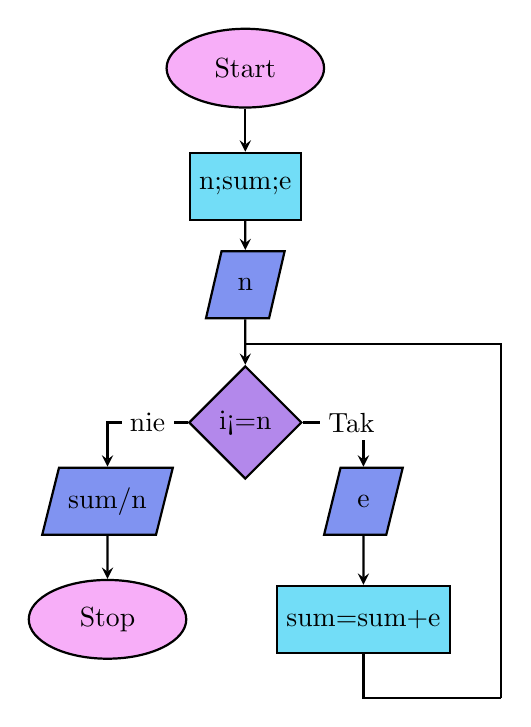
\begin{tikzpicture}
		\node [style=startstop] (0) at (0, 0) {Start};
		\node [style=io] (1) at (0, -2.75) {n};
		\node [style=process] (2) at (0, -1.5) {n;sum;e};
		\node [style=decision] (3) at (0, -4.5) {i<=n};
		\node [style=io] (4) at (1.5, -5.5) {e};
		\node [style=process] (5) at (1.5, -7) {sum=sum+e};
		\node [style=io] (6) at (-1.75, -5.5) {sum/n};
		\node [style=startstop] (7) at (-1.75, -7) {Stop};
		\node [style=none] (8) at (3.25, -8) {};
		\node [style=none] (9) at (0, -3.5) {};

        % node[pos=0.4,fill=white,inner sep=3]{nie};
		% node[pos=0.25,fill=white,inner sep=3]{Tak};

		\draw [style=arrow] (0) to (2);
		\draw [style=arrow] (2) to (1);
		\draw [style=arrow] (1) to (3);
		\draw [style=arrow] (3) -| (4)node[pos=0.4,fill=white,inner sep=3]{Tak};
		\draw [style=arrow] (4) to (5);
		\draw [style=con] (5) |- (8.center);
		\draw [style=con] (8.center) |- (9.center);
		\draw [style=arrow] (3) -| (6)node[pos=0.25,fill=white,inner sep=3]{nie};
		\draw [style=arrow] (6) to (7);
\end{tikzpicture}
\caption{2.5 flowchart}
    \label{flow5}
\end{figure}
    \end{flushleft}
D: \\
n, ilość liczb $\in$ $\mathbb{N}$\\
e, n'ta liczba ciągu $\in$ $\mathbb{R}$\\
W: strumień, średnia ciągu $\in$ $\mathbb{R}$
    \begin{flushright}
    \renewcommand{\thefigure}{5}
\begin{figure}[H]
    \centering 
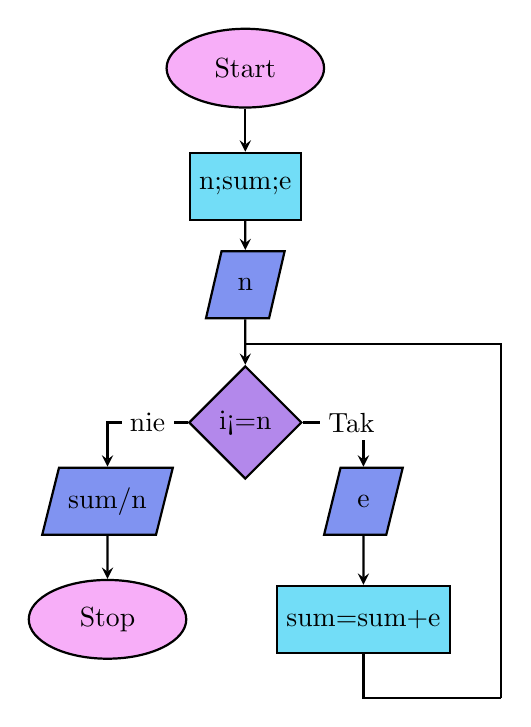
\begin{tikzpicture}
		\node [style=startstop] (0) at (0, 0) {Start};
		\node [style=io] (1) at (0, -2.75) {n};
		\node [style=process] (2) at (0, -1.5) {n;sum;e};
		\node [style=decision] (3) at (0, -4.5) {i<=n};
		\node [style=io] (4) at (1.5, -5.5) {e};
		\node [style=process] (5) at (1.5, -7) {sum=sum+e};
		\node [style=io] (6) at (-1.75, -5.5) {sum/n};
		\node [style=startstop] (7) at (-1.75, -7) {Stop};
		\node [style=none] (8) at (3.25, -8) {};
		\node [style=none] (9) at (0, -3.5) {};

        % node[pos=0.4,fill=white,inner sep=3]{nie};
		% node[pos=0.25,fill=white,inner sep=3]{Tak};

		\draw [style=arrow] (0) to (2);
		\draw [style=arrow] (2) to (1);
		\draw [style=arrow] (1) to (3);
		\draw [style=arrow] (3) -| (4)node[pos=0.4,fill=white,inner sep=3]{Tak};
		\draw [style=arrow] (4) to (5);
		\draw [style=con] (5) |- (8.center);
		\draw [style=con] (8.center) |- (9.center);
		\draw [style=arrow] (3) -| (6)node[pos=0.25,fill=white,inner sep=3]{nie};
		\draw [style=arrow] (6) to (7);
\end{tikzpicture}
\caption{2.5 flowchart}
    \label{flow5}
\end{figure}
    \end{flushright}    
\end{multicols}

\subsection*{2.6}
%----------------2.6------------------
\begin{multicols}{2}
  \begin{flushleft}
\begin{minted}[framesep=1mm, baselinestretch=1.,linenos]{cpp}
int n=0;cout<<"podaj n: ";cin>>n;
int l[3]= {0,0,0};int p=100;
for (int m=round(pow(75.8531-cos(-0.896604*n),\
cos(0.0903642*n-1.26534))-4.43137);m>0;p++)
{l[0]=floor(p/100);
l[1]=floor((p-l[0]*100)/10);
l[2]=p-(l[1]*10+l[0]*100);
if(l[0]+l[1]+l[2]==n){m--;cout<<p<<endl;}
}cout<<"liczbe możliwości: "<<i;
\end{minted}
    \end{flushleft}
D:n, cyfra $\in$ \{1,2,3...27\}\\
W:strumień, liczby spełniające wrunek\\
i ich ilość $\in$ \{100,101,102...999\}
\begin{flushright}


    \begin{minted}[framesep=1mm, baselinestretch=1.,linenos]{cpp}
int n=0;cout<<"podaj n: ";cin>>n;
int l[3]= {0,0,0};int p=100;
for (int m=round(pow(75.8531-cos(-0.896604*n),\
cos(0.0903642*n-1.26534))-4.43137);m>0;p++)
{l[0]=floor(p/100);
l[1]=floor((p-l[0]*100)/10);
l[2]=p-(l[1]*10+l[0]*100);
if(l[0]+l[1]+l[2]==n){m--;cout<<p<<endl;}
}cout<<"liczbe możliwości: "<<i;
\end{minted}
\end{flushright} 
\end{multicols}

\subsection*{2.7}
%----------------2.7------------------
\begin{multicols}{2}
  \begin{flushleft}
\begin{tikzpicture}
	\begin{pgfonlayer}{nodelayer}
		\node [style=startstop] (0) at (0, 0.25) {Start};
		\node [style=process] (1) at (0, -1.25) {d='N'};
		\node [style=process] (2) at (0, -3) {2.6};
		\node [style=io] (3) at (0, -4.75) {toupper(d)};
		\node [style=decision] (4) at (0, -6.75) {d='T'|| d='N'};
		\node [style=decision] (5) at (1.5, -8.5) {d!='N'};
		\node [style=startstop] (6) at (0, -9.75) {Stop};
		\node [style=none] (7) at (0, -2) {};
		\node [style=none] (8) at (2.75, -2) {};
		\node [style=none] (9) at (-1.75, -3.75) {};
		\node [style=none] (10) at (0, -3.75) {};
	\end{pgfonlayer}
	\begin{pgfonlayer}{edgelayer}
		\draw [style=arrow] (0) to (1);
		\draw [style=arrow] (1) to (2);
		\draw [style=arrow] (2) to (3);
		\draw [style=arrow] (3) to (4);
		\draw [style=arrow] (4) to (5);
		\draw [style=arrow] (5) to (6);
		\draw (5) to (8.center);
		\draw (8.center) to (7.center);
		\draw (4) to (9.center);
		\draw (9.center) to (10.center);
	\end{pgfonlayer}
\end{tikzpicture}

    \end{flushleft}
D:n, cyfra $\in$ \{1,2,3...27\}\\
W:strumień, liczby spełniające wrunek\\
i ich ilość $\in$ \{100,101,102...999\}
    \begin{flushright}
    \begin{minted}[framesep=1mm, baselinestretch=1.,linenos]{python}
import msvcrt as m
import sys
print('program do liczenie liczb trzy cyfrowych ktorych suma jest rowna n:')
while True:
    n=int(input('podaj n:'))
    sum=int(0)
    for a in range(1,10):
        for b in range(0,10):
            for c in range(0,10):
                if a+b+c==n:print(a*100+b*10+c,", ",end='');sum=sum+1
    print("\nliczb trzy czyfrowych o sumie ",n," jest: ",sum)
    while True:
        print('kontynować? T/N')
        s=m.getche().upper()
        if s==b'T':break
        elif s==b'N':sys.exit(0)
\end{minted}
    \end{flushright}    
\end{multicols}

\subsection*{2.8}
%----------------2.8------------------
\begin{multicols}{2}
  \begin{flushleft}
\begin{minted}[framesep=1mm, baselinestretch=1.,linenos]{cpp}
cout<<"program do liczenina średniaj z\
n liczb dwucyfrowych, dodatnich"<<endl;
float sum=0;float e=0;
cout<<"podaj n: ";int n=0;cin>>n;
for(int i=1;i<=n;i++)
{cin.clear();cin.sync();
cout<<"podaj "<<i<<" liczbe: ";
cin>>e;
if (cin.fail()||e<10||e>=100)
{cout<<"podana wartosc jest nie poprawna\
sprubuj ponownie"<<endl;i--;e=0;}
sum=sum+e;}
cout<<setprecision(2)<<"srednia "<<n<<"\
dwucyfrowych liczb jest rowna: "<<sum/n<<endl;
\end{minted}
    \end{flushleft}
D: \\
n, ilość liczb $\in$ $\mathbb{N}$\\
e, n'ta liczba ciągu $\in$ \{10,11,12...99\}\\
W: strumień, średnia ciągu $\in$ $\mathbb{R}$
    \begin{flushright}
    \begin{minted}[framesep=1mm, baselinestretch=1.,linenos]{cpp}
cout<<"program do liczenina średniaj z\
n liczb dwucyfrowych, dodatnich"<<endl;
float sum=0;float e=0;
cout<<"podaj n: ";int n=0;cin>>n;
for(int i=1;i<=n;i++)
{cin.clear();cin.sync();
cout<<"podaj "<<i<<" liczbe: ";
cin>>e;
if (cin.fail()||e<10||e>=100)
{cout<<"podana wartosc jest nie poprawna\
sprubuj ponownie"<<endl;i--;e=0;}
sum=sum+e;}
cout<<setprecision(2)<<"srednia "<<n<<"\
dwucyfrowych liczb jest rowna: "<<sum/n<<endl;
\end{minted}
    \end{flushright}    
\end{multicols}

\subsection*{2.9}
%----------------2.9------------------
\begin{multicols}{2}
  \begin{flushleft}
\begin{minted}[framesep=1mm, baselinestretch=1.,linenos]{python}
print('program do nwd i nww')
a=int(0)
b=int(0)
i=int(1)
while True:
    try:
        a=int(input('podaj a liczbe:'))
        break   
    except ValueError:print('zła wartość')
while True:
    try:
        b=int(input('podaj b liczbe:'))
        break   
    except ValueError:print('zła wartość')    
c=int(0)
x=a
y=b
print('test')
while b != 0:
    c = a % b
    a = b
    b = c
    print('test')
x=int((x*y)/a)
print("nwd:", a, "nww:", x)
\end{minted}
    \end{flushleft}
D:a i b, liczby do nww i nwd $\in$ $\mathbb{N}$\\
W:a i x, nww i nwd $\in$ $\mathbb{N}$
    \begin{flushright}
    \begin{minted}[framesep=1mm, baselinestretch=1.,linenos]{python}
print('program do nwd i nww')
a=int(0)
b=int(0)
i=int(1)
while True:
    try:
        a=int(input('podaj a liczbe:'))
        break   
    except ValueError:print('zła wartość')
while True:
    try:
        b=int(input('podaj b liczbe:'))
        break   
    except ValueError:print('zła wartość')    
c=int(0)
x=a
y=b
print('test')
while b != 0:
    c = a % b
    a = b
    b = c
    print('test')
x=int((x*y)/a)
print("nwd:", a, "nww:", x)
\end{minted}
    \end{flushright}    
\end{multicols}

\subsection*{2.10}
%----------------2.10------------------
\begin{multicols}{2}
  \begin{flushleft}
\begin{minted}[framesep=1mm, baselinestretch=1.,linenos]{cpp}
int a[2]={0,16};
string c[2]={"min","max"};
int i;int x;int y;int l=4;
cout<<"program tabliczka mno�enie od do.\n\
Program przymuje wartości <-15;15>"<<endl;  
while(i<2){
cout<<"podaj "<<c[i]<<": ";
cin.clear();cin.sync();
a[i]=0;cin>>a[i];
if(cin.fail()||abs(a[i])>15||a[0]>a[1])
{cout<<endl<<"podana wartość jest nie poprawna"<<endl;
i--;}i++;}system("cls");y=a[0];
while (y<=a[1])
{
    x=a[0];cout<<y;gotoxy(3,y-a[0]+2);
    cout<<"|";
    while (x<=a[1]){
        gotoxy((x-a[0]+1)*l,y-a[0]+2);
        cout<<y*x;
        x++;}
    cout<<endl;y++;
}
\end{minted}
    \end{flushleft}
D: a[], przedział tabliczki mnożenia $\in$ \{-15,-14,-13...15\}\\
W: strumień, tabliczka mnożenia od a[0] do a[1] $\in$ \{-225,-224,-223...225\}
    \begin{flushright}
    \begin{minted}[framesep=1mm, baselinestretch=1.,linenos]{cpp}
int a[2]={0,16};
string c[2]={"min","max"};
int i;int x;int y;int l=4;
cout<<"program tabliczka mno�enie od do.\n\
Program przymuje wartości <-15;15>"<<endl;  
while(i<2){
cout<<"podaj "<<c[i]<<": ";
cin.clear();cin.sync();
a[i]=0;cin>>a[i];
if(cin.fail()||abs(a[i])>15||a[0]>a[1])
{cout<<endl<<"podana wartość jest nie poprawna"<<endl;
i--;}i++;}system("cls");y=a[0];
while (y<=a[1])
{
    x=a[0];cout<<y;gotoxy(3,y-a[0]+2);
    cout<<"|";
    while (x<=a[1]){
        gotoxy((x-a[0]+1)*l,y-a[0]+2);
        cout<<y*x;
        x++;}
    cout<<endl;y++;
}
\end{minted}
    \end{flushright}    
\end{multicols}
\newpage

\subsection*{2.11}
%----------------2.11------------------
\begin{multicols}{2}
  \begin{flushleft}
\begin{minted}[framesep=1mm, baselinestretch=1.,linenos]{python}
print("program do szukania minimalne liczby z ciągu liczb dwu cyfrowych")
print("aby zakończyć podawanie ciągu podaj liczbę 0")
i = 0
a=1
min_val = 100
while a != 0:
    
    i += 1
    while True:
        try:
            a=int(input('podaj liczbe:'))
            if abs(a) > 10 and abs(a) < 99:break
            if a==0:break   
            print("podana wartość jest nie poprawna")
        except ValueError:
            print('zła wartość')
            i=i-1
    if a == 0:
        break
    elif a < min_val: min_val=a
print("minimalną liczbą z ciągu:")
if min_val == 100:
    print("najmniejsza liczba ciągu należy do zbioru pustego")
else:
    print("jest: ", min_val)
\end{minted}
    \end{flushleft}
D: a, n'ta liczba ciągu $\in$ $\mathbb{R}$\\
W: min, najmniejszu element ciągu $\in$ $\mathbb{R}$
    \begin{flushright}
    \begin{minted}[framesep=1mm, baselinestretch=1.,linenos]{python}
print("program do szukania minimalne liczby z ciągu liczb dwu cyfrowych")
print("aby zakończyć podawanie ciągu podaj liczbę 0")
i = 0
a=1
min_val = 100
while a != 0:
    
    i += 1
    while True:
        try:
            a=int(input('podaj liczbe:'))
            if abs(a) > 10 and abs(a) < 99:break
            if a==0:break   
            print("podana wartość jest nie poprawna")
        except ValueError:
            print('zła wartość')
            i=i-1
    if a == 0:
        break
    elif a < min_val: min_val=a
print("minimalną liczbą z ciągu:")
if min_val == 100:
    print("najmniejsza liczba ciągu należy do zbioru pustego")
else:
    print("jest: ", min_val)
\end{minted}
    \end{flushright}    
\end{multicols}

\subsection*{2.12}
%----------------2.12------------------
\begin{multicols}{2}
  \begin{flushleft}
\begin{minted}[framesep=1mm, baselinestretch=1.,linenos]{cpp}
cout<<"program do nwd i nww"<<endl;  
int i;
char l='a';
int g[2]={0,0};      
while(i<2){
cout<<"podaj "<<l<<": ";
cin.clear();cin.sync();
g[i]=0;cin>>g[i];
if(cin.fail())
{cout<<endl<<"podana wartość jest nie poprawna"\
<<endl;i--;l--;}
i++;l++;}	
int a=abs(g[0]);int x=a;
int b=abs(g[1]);int y=b;     
while(a!=b)
{
	if(a>b){a=a-b;}
	else{b=b-a;}
}
x=(x*y)/a;
cout<<"nwd:"<<a<<" nww:"<<x<<endl;
\end{minted}
    \end{flushleft}
D:a i b, liczby do nww i nwd $\in$ $\mathbb{N}$\\
W:a i x, nww i nwd $\in$ $\mathbb{N}$
    \begin{flushright}
    \begin{minted}[framesep=1mm, baselinestretch=1.,linenos]{cpp}
cout<<"program do nwd i nww"<<endl;  
int i;
char l='a';
int g[2]={0,0};      
while(i<2){
cout<<"podaj "<<l<<": ";
cin.clear();cin.sync();
g[i]=0;cin>>g[i];
if(cin.fail())
{cout<<endl<<"podana wartość jest nie poprawna"\
<<endl;i--;l--;}
i++;l++;}	
int a=abs(g[0]);int x=a;
int b=abs(g[1]);int y=b;     
while(a!=b)
{
	if(a>b){a=a-b;}
	else{b=b-a;}
}
x=(x*y)/a;
cout<<"nwd:"<<a<<" nww:"<<x<<endl;
\end{minted}
    \end{flushright}    
\end{multicols}
\newpage
\subsection*{2.13}
%----------------2.13------------------
\begin{multicols}{2}
  \begin{flushleft}
  \begin{minted}[framesep=1mm, baselinestretch=1.,linenos]{cpp}
cout<<"program liczenia silni z n"<<endl;   
int i;int n;long long s;
i=1;n=1;s=1;
cout<<"podaj n:";
cin.clear();cin.sync();cin>>n;
while(i<=n){s=s*i;i++;}
cout<<"silna z n jest równa:"<<s<<endl;
\end{minted}
D: n, liczba do silni $\in$ $\mathbb{N}$\\
W: s, silnia n $\in$ $\mathbb{N}$
\begin{minted}[framesep=1mm, baselinestretch=1.,linenos]{text}
Zarezerwuj miejsce dla i, n, s
i, n, s równają się 1 
Zapytaj użytkownika o n
s jest równe iloczynowi i oraz s
zwiększ i o jeden
jeżeli i jest nie mniejsze od n wróć do pkt.4
przekaż s do strumienia  
\end{minted}
    \end{flushleft}

    \begin{flushright}
    \begin{minted}[framesep=1mm, baselinestretch=1.,linenos]{cpp}
cout<<"program liczenia silni z n"<<endl;   
int i;int n;long long s;
i=1;n=1;s=1;
cout<<"podaj n:";
cin.clear();cin.sync();cin>>n;
while(i<=n){s=s*i;i++;}
cout<<"silna z n jest równa:"<<s<<endl;
\end{minted}
    \end{flushright}    
\end{multicols}

\subsection*{2.14}
%----------------2.14------------------
\begin{multicols}{2}
  \begin{flushleft}
\begin{minted}[framesep=1mm, baselinestretch=1.,linenos]{cpp}
cout<<endl<<"program do liczenie n liczby fibonacciego"<<endl;  
cout<<"\npodaj n:";
int n = 0;
cin>>n;
if(cin.fail()){r=false;cout<<endl<<"podana wartość jest nie poprawna"<<endl;}
int i = 0;
double a=0;double b=1;double c=0;
while (n>i)
{c=a+b;a=b;b=c;i++;}
cout<<n<<" liczba ciagu fibonacciego jest rowna:"<<a<<endl;
\end{minted}
D: n, index liczby fibonaciego $\in$ $\mathbb{N}$\\
W: s, n'ta liczba ciągu fibonaciego $\in$ $\mathbb{N}$
\end{flushleft}
\begin{minipage}{3cm}
%\vspace{1cm}
\begin{minted}[framesep=1mm, baselinestretch=1.,linenos]{text}
Zarezerwuj miejsce dla n, i, a, b, c
b równa się 1 
c jest równe sumie a i b
a równa się b
b równa się c 
zwiększ i o jeden
jeżeli n jest większe od i to wróć do 3 kroku
przekaż a do strumienia
\end{minted}   
\end{minipage}
\begin{flushright}
\end{flushright}    
\end{multicols}
\hspace{3cm}
\begin{minipage}{3cm}
\begin{minted}[framesep=1mm, baselinestretch=1.,linenos]{cpp}
cout<<endl<<"program do liczenie n liczby fibonacciego"<<endl;  
cout<<"\npodaj n:";
int n = 0;
cin>>n;
if(cin.fail()){r=false;cout<<endl<<"podana wartość jest nie poprawna"<<endl;}
int i = 0;
double a=0;double b=1;double c=0;
while (n>i)
{c=a+b;a=b;b=c;i++;}
cout<<n<<" liczba ciagu fibonacciego jest rowna:"<<a<<endl;
\end{minted}  
\end{minipage}

    


\newpage
\subsection*{2.15}
%----------------2.15------------------
\begin{multicols}{2}
  \begin{flushleft}


D: n, liczba do sprawdzenia $\in$ $\mathbb{N}$\\
W: odp, czy liczba jest pierwsza $\in$ $\{"tak";"nie"\}$

\hspace{0.4cm}
\begin{minipage}{3cm}
\vspace{0.6cm}
\small
\begin{minted}[framesep=1mm, baselinestretch=1.,linenos]{text}
Odp równa się „tak”, i równa się 3 a n równa się jeden
Zapytaj użytkownika o n
Jeżeli  n jest podzielne przez 2 to odp przyjmuje wartość „nie”
Jeżeli reszta n/i jest 0 to odp przyjmuje wartość „nie”
Zwiększ i o 2
Jeżeli i jest mniejszy od pierwiastku z n to idź do czwartego kroku 
Przekaż odp do strumienia 
\end{minted}
\normalsize
\begin{minted}[framesep=1mm, baselinestretch=1.,linenos]{cpp}
cout<<"program do sprawdzania czy liczba jest pierwsza"<<endl;  
int i=3;int n=1;string odp="tak";
cout<<"podaj n:";
cin.clear();cin.sync();cin>>n;
if (n%2==0 && n!=2){odp="nie";}
while(i<sqrt(n))
{
    if(n%i==0){odp="nie";break;}
    i=i+2;
}
cout<<odp<<endl;
\end{minted}
\end{minipage}

    \end{flushleft}

    \begin{flushright}
    \begin{tikzpicture}
	\begin{pgfonlayer}{nodelayer}
		\node [style=startstop] (0) at (0, 0) {Start};
		\node [style=process] (1) at (0, -1.5) {i=2;n=1;odp="tak"};
		\node [style=io] (2) at (0, -2.75) {n};
		\node [style=decision] (3) at (0, -5) {i<sqrt(n)};
		\node [style=decision] (4) at (1.5, -6.75) {n\%i==0};
		\node [style=process] (6) at (2.75, -8) {odp="nie"};
		\node [style=process] (8) at (0.25, -8) {i++};
		\node [style=none] (9) at (2.75, -8.75) {};
		\node [style=none] (10) at (0, -3.5) {};
		\node [style=none] (11) at (3.75, -9.75) {};
		\node [style=startstop] (12) at (-2.5, -7.5) {Stop};
		\node [style=io] (14) at (-2.5, -6) {odp};
		\node [style=none] (15) at (0.5, -8.75) {};
		\node [style=none] (16) at (0, -8.75) {};
		\node [style=none] (17) at (-1.25, -5) {};
	\end{pgfonlayer}
	\begin{pgfonlayer}{edgelayer}
		\draw [style=arrow] (0) to (1);
		\draw [style=arrow] (1) to (2);
		\draw [style=arrow] (2) to (3);
		\draw [style=arrow] (3) to (4);
		\draw [style=arrow] (4) to (6);
		\draw [style=con] (6) to (9.center);
		\draw [style=con] (8) to (11.center);
		\draw [style=arrow] (4) to (8);
		\draw [style=arrow] (3) to (14);
		\draw [style=arrow] (14) to (12);
		\draw [style=con] (11.center) to (10.center);
		\draw [style=con] (9.center) to (15.center);
		\draw [style=con, in=-90, out=-90, looseness=1.75] (15.center) to (16.center);
		\draw [style=arrow] (16.center) to (17.center);
	\end{pgfonlayer}
\end{tikzpicture}

   
    \end{flushright}    
\end{multicols}
\subsection*{2.16}

%----------------2.16------------------
\normalsize
\begin{multicols}{2}
  \begin{flushleft}
D: n, liczba $\in$ $\mathbb{N}_0$\\
W: s, ilość cyfr w n $\in$ $\mathbb{N}_0$

\hspace{0.4cm}
\begin{minipage}{3cm}
\vspace{0.6cm}
\begin{minted}[framesep=1mm, baselinestretch=1.,linenos]{text}
Zarezerwuj miejsce dla n i s 
Zapytaj użytkownika o n
Dodaj do s resztę dzielenia dziesiętnego z n
Podziel n przez dziesięć 
Jeżeli n nie równa się zero idź do kroku 3
Przekaż s do strumienia 
\end{minted}
\begin{minted}[framesep=1mm, baselinestretch=1.,linenos]{python}
import math

print('program do sprawdzania jaka jest suma cyfr n')
s=int(0)
n=int(1)
while True:
    try:
        n=round(int(input('podaj a liczbe:')))
        break   
    except ValueError:print('zła wartość')

while True:
    if n==0:
        break
    s=s+n%10
    n=round(n/10)
print('Suma wszystkich cyfr to', s)
\end{minted}
\end{minipage}


    \end{flushleft}

    \begin{flushright}
    
    \begin{tikzpicture}
	\begin{pgfonlayer}{nodelayer}
		\node [style=startstop] (0) at (0, 0) {Start};
		\node [style=process] (1) at (0, -1.5) {n=1;s=0};
		\node [style=io] (2) at (0, -3) {n};
		\node [style=decision] (3) at (0, -5) {n==0};
		\node [style=io] (4) at (1.25, -6) {s};
		\node [style=startstop] (5) at (1.25, -7.5) {Stop};
		\node [style=process] (6) at (-1.5, -6.25) {s=s+n\%10; n=n/10};
		\node [style=none] (7) at (-2.75, -7.5) {};
		\node [style=none] (8) at (0, -3.75) {};
	\end{pgfonlayer}
	\begin{pgfonlayer}{edgelayer}
		\draw [style=arrow] (0) to (1);
		\draw [style=arrow] (1) to (2);
		\draw [style=arrow] (2) to (3);
		\draw [style=arrow] (3) to (4);
		\draw [style=arrow] (4) to (5);
		\draw [style=arrow] (3) to (6);
		\draw [style=con] (6) to (7.center);
		\draw [style=con] (7.center) to (8.center);
	\end{pgfonlayer}
\end{tikzpicture}

    \end{flushright}    
\end{multicols}
\newpage
%-------------alternatywne rozwiązamnia
\section{Alternatywne rozwiązania}
\begin{center}
\large \textbf{python}
\end{center}
\small
\begin{multicols}{2}
\begin{flushleft}
    \hspace{1cm}
    \begin{minipage}{3cm}
        \subsection*{2.1}
        \begin{minted}[framesep=1mm, baselinestretch=1.,linenos]{python}
import msvcrt
def dis(argument):
    switcher = {
        'E': print("EUR:",saldo/e,'\n'),
        'U': print("USD:",saldo/u,'\n'),
        'F': print("CHF:",saldo/f,'\n'),
        'P': print("PLN:",saldo/p,'\n'),
    }
e=4;u=3;f=5;p=1
saldo=int(input('Ile masz pieniedzy:'))
print('w jakiej walucie')
c=msvcrt.getche().upper()
print(c)
match c:
    case b'E': 
        saldo=saldo*e; dis('E'),
    case b'U':
        saldo=saldo*u; dis('U'),
    case b'F':
        saldo=saldo*f; dis('F'),
    case b'P':
        saldo=saldo*p; dis('p'),
\end{minted}    

        \subsection*{2.2}
        \begin{minted}[framesep=1mm, baselinestretch=1.,linenos]{cpp}
int a;char fig; 
cout<<"podaj długość boku:"<<endl;
cin>>a;cout<<"dostępne figury:\n1.kwadrat\
\n2.trójkąt\n3.pięcokąt\n4.sześciokąt";
fig=getch();
switch (fig)
{case '1':
cout<<"\nobwód jest równy "<<a*4<<"\
a pole "<<a*a;break;
case '2':
cout<<"\nobwód jest równy "<<a*3<<"\
a pole "<<a*a*sqrt(3)/4;break;
case '3':
cout<<"\nobwód jest równy "<<a*5<<"\
a pole "<<(sqrt(25+10*sqrt(5))/4)*a*a;break;
case '4':
cout<<"\nobwód jest równy "<<a*6<<"\
a pole "<<(a*a*sqrt(3)/4)*6;break;        
default:
cout<<"podana opcja jest zła";break;}
\end{minted}

        \subsection*{2.3}
        \renewcommand{\thefigure}{3}
\begin{figure}[H]
    \centering 
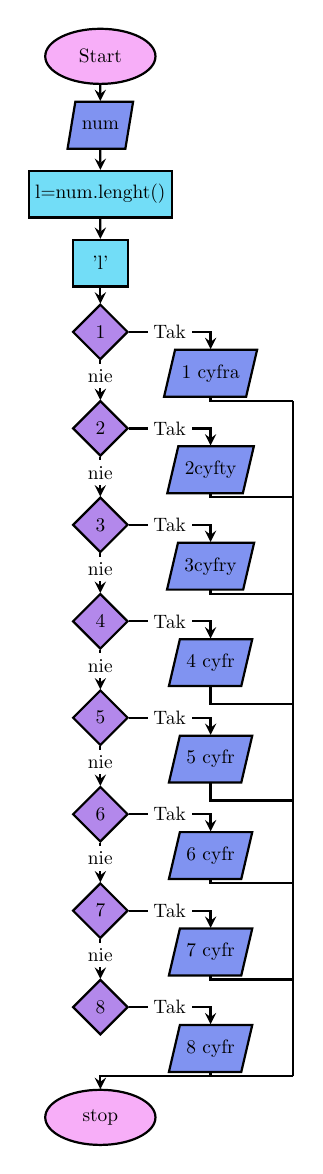
\begin{tikzpicture}[scale=0.7,transform shape]
		\node [style=startstop] (0) at (0, 0) {Start};
		\node [style=io] (1) at (0, -1.25) {num};
		\node [style=process] (3) at (0, -3.75) {'l'};
		\node [style=decision] (4) at (0, -5) {1};
		\node [style=decision] (5) at (0, -6.75) {2};
		\node [style=decision] (6) at (0, -8.5) {3};
		\node [style=decision] (7) at (0, -10.25) {4};
		\node [style=process] (8) at (0, -2.5) {l=num.lenght()};
		\node [style=decision] (9) at (0, -12) {5};
		\node [style=decision] (10) at (0, -13.75) {6};
		\node [style=decision] (11) at (0, -15.5) {7};
		\node [style=decision] (12) at (0, -17.25) {8};
		\node [style=io] (14) at (2, -5.75) {1 cyfra};
		\node [style=io] (15) at (2, -7.5) {2cyfty};
		\node [style=io] (16) at (2, -9.25) {3cyfry};
		\node [style=io] (17) at (2, -11) {4 cyfr};
		\node [style=io] (18) at (2, -12.75) {5 cyfr};
		\node [style=io] (19) at (2, -14.5) {6 cyfr};
		\node [style=io] (20) at (2, -16.25) {7 cyfr};
		\node [style=io] (21) at (2, -18) {8 cyfr};
		\node [style=startstop] (22) at (0, -19.25) {stop};
		\node [style=none] (23) at (3.5, -6.25) {};
		\node [style=none] (24) at (3.5, -8) {};
		\node [style=none] (25) at (3.5, -9.75) {};
		\node [style=none] (26) at (3.5, -11.75) {};
		\node [style=none] (27) at (3.5, -13.5) {};
		\node [style=none] (28) at (3.5, -15) {};
		\node [style=none] (29) at (3.5, -16.75) {};
		\node [style=none] (30) at (3.5, -18.5) {};

%\draw [arrow] (c3) -- (c4)node[pos=0.4,fill=white,inner sep=3]{nie};
%\draw [arrow] (c1) -| (p1)node[pos=0.25,fill=white,inner sep=3]{Tak};

		\draw [style=arrow] (0) to (1);
		\draw [style=arrow] (1) to (8);
		\draw [style=arrow] (8) to (3);
		\draw [style=arrow] (3) to (4);
		\draw [style=arrow] (4) -- (5)node[pos=0.4,fill=white,inner sep=3]{nie};
		\draw [style=arrow] (5) -- (6)node[pos=0.4,fill=white,inner sep=3]{nie};
		\draw [style=arrow] (6) -- (7)node[pos=0.4,fill=white,inner sep=3]{nie};
		\draw [style=arrow] (7) -- (9)node[pos=0.4,fill=white,inner sep=3]{nie};
		\draw [style=arrow] (9) -- (10)node[pos=0.4,fill=white,inner sep=3]{nie};
		\draw [style=arrow] (10) -- (11)node[pos=0.4,fill=white,inner sep=3]{nie};
		\draw [style=arrow] (11) -- (12)node[pos=0.4,fill=white,inner sep=3]{nie};
		\draw [style=arrow] (4) -| (14)node[pos=0.25,fill=white,inner sep=3]{Tak};
		\draw [style=arrow] (5) -| (15)node[pos=0.25,fill=white,inner sep=3]{Tak};
		\draw [style=arrow] (6) -| (16)node[pos=0.25,fill=white,inner sep=3]{Tak};
		\draw [style=arrow] (7) -| (17)node[pos=0.25,fill=white,inner sep=3]{Tak};
		\draw [style=arrow] (9) -| (18)node[pos=0.25,fill=white,inner sep=3]{Tak};
		\draw [style=arrow] (10) -| (19)node[pos=0.25,fill=white,inner sep=3]{Tak};
		\draw [style=arrow] (11) -| (20)node[pos=0.25,fill=white,inner sep=3]{Tak};
		\draw [style=arrow] (12) -| (21)node[pos=0.25,fill=white,inner sep=3]{Tak};
		\draw [style=con] (14) |- (23.center);
		\draw [style=con] (15) |- (24.center);
		\draw [style=con] (16) |- (25.center);
		\draw [style=con] (17) |- (26.center);
		\draw [style=con] (18) |- (27.center);
		\draw [style=con] (19) |- (28.center);
		\draw [style=con] (20) |- (29.center);
		\draw [style=con] (21) |- (30.center);
		\draw [style=con] (23.center) to (30.center);
		\draw [style=arrow] (30.center) -| (22);
\end{tikzpicture}
\caption{2.3 flowchart}
    \label{flow3}
\end{figure}   
        \end{minipage}  
\end{flushleft}
\subsection*{2.4}
\begin{minted}[framesep=1mm, baselinestretch=1.,linenos]{cpp}
cout<<"ile jest liczb podzielnych\
przez c w przdziale a-b"<<endl;  
cout<<"podaj a:";int a=0;cin>>a;
cout<<"podaj b:";int b=0;cin>>b;
cout<<"podaj c:";int c=0;cin>>c;
cout<<"przdzial "<<a<<" ; "<<b<<" zawiera ";
bool t=a%c;
a=a+(c*t-(a%c+c)%c);
b=b-(b%c+c)%c;
int n=(b-a)/c+1;
cout<<n<<" liczb podzielnych przez "<<c<<endl;
for(int i=0;i<n;i++){cout<<a+c*i<<", ";}
\end{minted}
\subsection*{2.5}
\renewcommand{\thefigure}{5}
\begin{figure}[H]
    \centering 
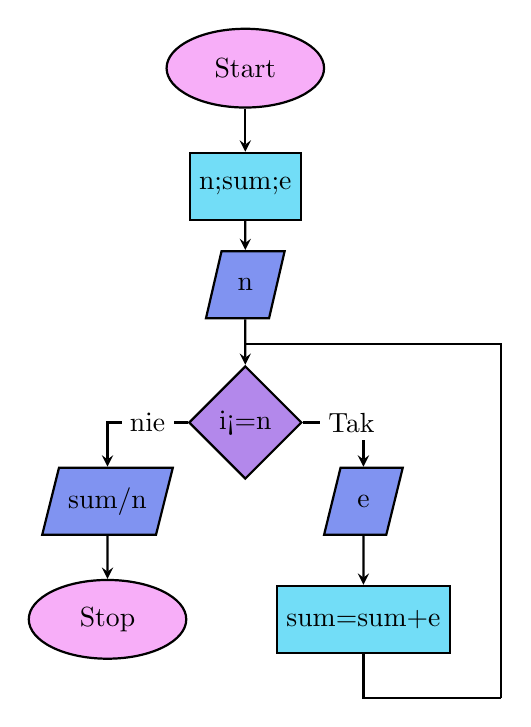
\begin{tikzpicture}
		\node [style=startstop] (0) at (0, 0) {Start};
		\node [style=io] (1) at (0, -2.75) {n};
		\node [style=process] (2) at (0, -1.5) {n;sum;e};
		\node [style=decision] (3) at (0, -4.5) {i<=n};
		\node [style=io] (4) at (1.5, -5.5) {e};
		\node [style=process] (5) at (1.5, -7) {sum=sum+e};
		\node [style=io] (6) at (-1.75, -5.5) {sum/n};
		\node [style=startstop] (7) at (-1.75, -7) {Stop};
		\node [style=none] (8) at (3.25, -8) {};
		\node [style=none] (9) at (0, -3.5) {};

        % node[pos=0.4,fill=white,inner sep=3]{nie};
		% node[pos=0.25,fill=white,inner sep=3]{Tak};

		\draw [style=arrow] (0) to (2);
		\draw [style=arrow] (2) to (1);
		\draw [style=arrow] (1) to (3);
		\draw [style=arrow] (3) -| (4)node[pos=0.4,fill=white,inner sep=3]{Tak};
		\draw [style=arrow] (4) to (5);
		\draw [style=con] (5) |- (8.center);
		\draw [style=con] (8.center) |- (9.center);
		\draw [style=arrow] (3) -| (6)node[pos=0.25,fill=white,inner sep=3]{nie};
		\draw [style=arrow] (6) to (7);
\end{tikzpicture}
\caption{2.5 flowchart}
    \label{flow5}
\end{figure}
\vspace{7.05cm}
\subsection*{2.6}
\begin{minted}[framesep=1mm, baselinestretch=1.,linenos]{cpp}
int n=0;cout<<"podaj n: ";cin>>n;
int l[3]= {0,0,0};int p=100;
for (int m=round(pow(75.8531-cos(-0.896604*n),\
cos(0.0903642*n-1.26534))-4.43137);m>0;p++)
{l[0]=floor(p/100);
l[1]=floor((p-l[0]*100)/10);
l[2]=p-(l[1]*10+l[0]*100);
if(l[0]+l[1]+l[2]==n){m--;cout<<p<<endl;}
}cout<<"liczbe możliwości: "<<i;
\end{minted}
\end{multicols}
\newpage

\begin{multicols}{2}
\begin{flushleft}
    \hspace{1cm}
    \begin{minipage}{3cm}
        \subsection*{2.7}
        \begin{tikzpicture}
	\begin{pgfonlayer}{nodelayer}
		\node [style=startstop] (0) at (0, 0.25) {Start};
		\node [style=process] (1) at (0, -1.25) {d='N'};
		\node [style=process] (2) at (0, -3) {2.6};
		\node [style=io] (3) at (0, -4.75) {toupper(d)};
		\node [style=decision] (4) at (0, -6.75) {d='T'|| d='N'};
		\node [style=decision] (5) at (1.5, -8.5) {d!='N'};
		\node [style=startstop] (6) at (0, -9.75) {Stop};
		\node [style=none] (7) at (0, -2) {};
		\node [style=none] (8) at (2.75, -2) {};
		\node [style=none] (9) at (-1.75, -3.75) {};
		\node [style=none] (10) at (0, -3.75) {};
	\end{pgfonlayer}
	\begin{pgfonlayer}{edgelayer}
		\draw [style=arrow] (0) to (1);
		\draw [style=arrow] (1) to (2);
		\draw [style=arrow] (2) to (3);
		\draw [style=arrow] (3) to (4);
		\draw [style=arrow] (4) to (5);
		\draw [style=arrow] (5) to (6);
		\draw (5) to (8.center);
		\draw (8.center) to (7.center);
		\draw (4) to (9.center);
		\draw (9.center) to (10.center);
	\end{pgfonlayer}
\end{tikzpicture}
    

        \subsection*{2.8}
        \begin{minted}[framesep=1mm, baselinestretch=1.,linenos]{cpp}
cout<<"program do liczenina średniaj z\
n liczb dwucyfrowych, dodatnich"<<endl;
float sum=0;float e=0;
cout<<"podaj n: ";int n=0;cin>>n;
for(int i=1;i<=n;i++)
{cin.clear();cin.sync();
cout<<"podaj "<<i<<" liczbe: ";
cin>>e;
if (cin.fail()||e<10||e>=100)
{cout<<"podana wartosc jest nie poprawna\
sprubuj ponownie"<<endl;i--;e=0;}
sum=sum+e;}
cout<<setprecision(2)<<"srednia "<<n<<"\
dwucyfrowych liczb jest rowna: "<<sum/n<<endl;
\end{minted}
        
        \subsection*{2.9}
        \begin{minted}[framesep=1mm, baselinestretch=1.,linenos]{python}
print('program do nwd i nww')
a=int(0)
b=int(0)
i=int(1)
while True:
    try:
        a=int(input('podaj a liczbe:'))
        break   
    except ValueError:print('zła wartość')
while True:
    try:
        b=int(input('podaj b liczbe:'))
        break   
    except ValueError:print('zła wartość')    
c=int(0)
x=a
y=b
print('test')
while b != 0:
    c = a % b
    a = b
    b = c
    print('test')
x=int((x*y)/a)
print("nwd:", a, "nww:", x)
\end{minted}
 
        \end{minipage}  
\end{flushleft}
\begin{minipage}{3cm}
\vspace{10cm}
\subsection*{2.10}
\begin{minted}[framesep=1mm, baselinestretch=1.,linenos]{cpp}
int a[2]={0,16};
string c[2]={"min","max"};
int i;int x;int y;int l=4;
cout<<"program tabliczka mno�enie od do.\n\
Program przymuje wartości <-15;15>"<<endl;  
while(i<2){
cout<<"podaj "<<c[i]<<": ";
cin.clear();cin.sync();
a[i]=0;cin>>a[i];
if(cin.fail()||abs(a[i])>15||a[0]>a[1])
{cout<<endl<<"podana wartość jest nie poprawna"<<endl;
i--;}i++;}system("cls");y=a[0];
while (y<=a[1])
{
    x=a[0];cout<<y;gotoxy(3,y-a[0]+2);
    cout<<"|";
    while (x<=a[1]){
        gotoxy((x-a[0]+1)*l,y-a[0]+2);
        cout<<y*x;
        x++;}
    cout<<endl;y++;
}
\end{minted}
\end{minipage}
\end{multicols}
\newpage
\begin{multicols}{2}
\begin{flushleft}
    \hspace{1cm}
    \begin{minipage}{3cm}
        \subsection*{2.11}
        \begin{minted}[framesep=1mm, baselinestretch=1.,linenos]{python}
print("program do szukania minimalne liczby z ciągu liczb dwu cyfrowych")
print("aby zakończyć podawanie ciągu podaj liczbę 0")
i = 0
a=1
min_val = 100
while a != 0:
    
    i += 1
    while True:
        try:
            a=int(input('podaj liczbe:'))
            if abs(a) > 10 and abs(a) < 99:break
            if a==0:break   
            print("podana wartość jest nie poprawna")
        except ValueError:
            print('zła wartość')
            i=i-1
    if a == 0:
        break
    elif a < min_val: min_val=a
print("minimalną liczbą z ciągu:")
if min_val == 100:
    print("najmniejsza liczba ciągu należy do zbioru pustego")
else:
    print("jest: ", min_val)
\end{minted}    

        \subsection*{2.12}
        \begin{minted}[framesep=1mm, baselinestretch=1.,linenos]{cpp}
cout<<"program do nwd i nww"<<endl;  
int i;
char l='a';
int g[2]={0,0};      
while(i<2){
cout<<"podaj "<<l<<": ";
cin.clear();cin.sync();
g[i]=0;cin>>g[i];
if(cin.fail())
{cout<<endl<<"podana wartość jest nie poprawna"\
<<endl;i--;l--;}
i++;l++;}	
int a=abs(g[0]);int x=a;
int b=abs(g[1]);int y=b;     
while(a!=b)
{
	if(a>b){a=a-b;}
	else{b=b-a;}
}
x=(x*y)/a;
cout<<"nwd:"<<a<<" nww:"<<x<<endl;
\end{minted}
        
        \subsection*{2.13}
        \begin{minted}[framesep=1mm, baselinestretch=1.,linenos]{cpp}
cout<<"program liczenia silni z n"<<endl;   
int i;int n;long long s;
i=1;n=1;s=1;
cout<<"podaj n:";
cin.clear();cin.sync();cin>>n;
while(i<=n){s=s*i;i++;}
cout<<"silna z n jest równa:"<<s<<endl;
\end{minted}
 
        \end{minipage}  
\end{flushleft}
\begin{minipage}{3cm}
\vspace{10.81cm}
\subsection*{2.14}
\begin{minted}[framesep=1mm, baselinestretch=1.,linenos]{cpp}
cout<<endl<<"program do liczenie n liczby fibonacciego"<<endl;  
cout<<"\npodaj n:";
int n = 0;
cin>>n;
if(cin.fail()){r=false;cout<<endl<<"podana wartość jest nie poprawna"<<endl;}
int i = 0;
double a=0;double b=1;double c=0;
while (n>i)
{c=a+b;a=b;b=c;i++;}
cout<<n<<" liczba ciagu fibonacciego jest rowna:"<<a<<endl;
\end{minted}
\end{minipage}
\end{multicols}
\newpage
\begin{multicols}{2}
\hspace{0.4cm}
\begin{minipage}{3cm}
\subsection*{2.15}
\begin{tikzpicture}
	\begin{pgfonlayer}{nodelayer}
		\node [style=startstop] (0) at (0, 0) {Start};
		\node [style=process] (1) at (0, -1.5) {i=2;n=1;odp="tak"};
		\node [style=io] (2) at (0, -2.75) {n};
		\node [style=decision] (3) at (0, -5) {i<sqrt(n)};
		\node [style=decision] (4) at (1.5, -6.75) {n\%i==0};
		\node [style=process] (6) at (2.75, -8) {odp="nie"};
		\node [style=process] (8) at (0.25, -8) {i++};
		\node [style=none] (9) at (2.75, -8.75) {};
		\node [style=none] (10) at (0, -3.5) {};
		\node [style=none] (11) at (3.75, -9.75) {};
		\node [style=startstop] (12) at (-2.5, -7.5) {Stop};
		\node [style=io] (14) at (-2.5, -6) {odp};
		\node [style=none] (15) at (0.5, -8.75) {};
		\node [style=none] (16) at (0, -8.75) {};
		\node [style=none] (17) at (-1.25, -5) {};
	\end{pgfonlayer}
	\begin{pgfonlayer}{edgelayer}
		\draw [style=arrow] (0) to (1);
		\draw [style=arrow] (1) to (2);
		\draw [style=arrow] (2) to (3);
		\draw [style=arrow] (3) to (4);
		\draw [style=arrow] (4) to (6);
		\draw [style=con] (6) to (9.center);
		\draw [style=con] (8) to (11.center);
		\draw [style=arrow] (4) to (8);
		\draw [style=arrow] (3) to (14);
		\draw [style=arrow] (14) to (12);
		\draw [style=con] (11.center) to (10.center);
		\draw [style=con] (9.center) to (15.center);
		\draw [style=con, in=-90, out=-90, looseness=1.75] (15.center) to (16.center);
		\draw [style=arrow] (16.center) to (17.center);
	\end{pgfonlayer}
\end{tikzpicture}
  
\end{minipage}

\subsection*{2.16}
\begin{tikzpicture}
	\begin{pgfonlayer}{nodelayer}
		\node [style=startstop] (0) at (0, 0) {Start};
		\node [style=process] (1) at (0, -1.5) {n=1;s=0};
		\node [style=io] (2) at (0, -3) {n};
		\node [style=decision] (3) at (0, -5) {n==0};
		\node [style=io] (4) at (1.25, -6) {s};
		\node [style=startstop] (5) at (1.25, -7.5) {Stop};
		\node [style=process] (6) at (-1.5, -6.25) {s=s+n\%10; n=n/10};
		\node [style=none] (7) at (-2.75, -7.5) {};
		\node [style=none] (8) at (0, -3.75) {};
	\end{pgfonlayer}
	\begin{pgfonlayer}{edgelayer}
		\draw [style=arrow] (0) to (1);
		\draw [style=arrow] (1) to (2);
		\draw [style=arrow] (2) to (3);
		\draw [style=arrow] (3) to (4);
		\draw [style=arrow] (4) to (5);
		\draw [style=arrow] (3) to (6);
		\draw [style=con] (6) to (7.center);
		\draw [style=con] (7.center) to (8.center);
	\end{pgfonlayer}
\end{tikzpicture}
   
\end{multicols}




%--------------Programy użyte----------
\section{Programy użyte do wykonoania zadań}  
\LaTeX, tikzit, firefox, overleaf, dev c++, c++, python, visual studio code, notepad++, git, github, Sumatra PDF, Total comander  
\section{Wnioski i uwagi} 
\begin{center}
 \large{Zadanie mi się bardzo podobało i nie mam żadnych uwag.}   
\end{center}
 
\end{document}
